\chapter{Suite numériques}

\section{La raisonnement par récurrence}
\subsection{Illustration}
\begin{minipage}[c]{0.47\textwidth}
		\textbf{Question :} quelles sont les deux conditions pour que tous les dominos se renversent ?
		
		\textbf{Réponse :} on renverse le premier domino et on s'assure que chaque domino renverse le suivant.
	
\end{minipage}
\hfill
\begin{minipage}[c]{0.47\textwidth}
	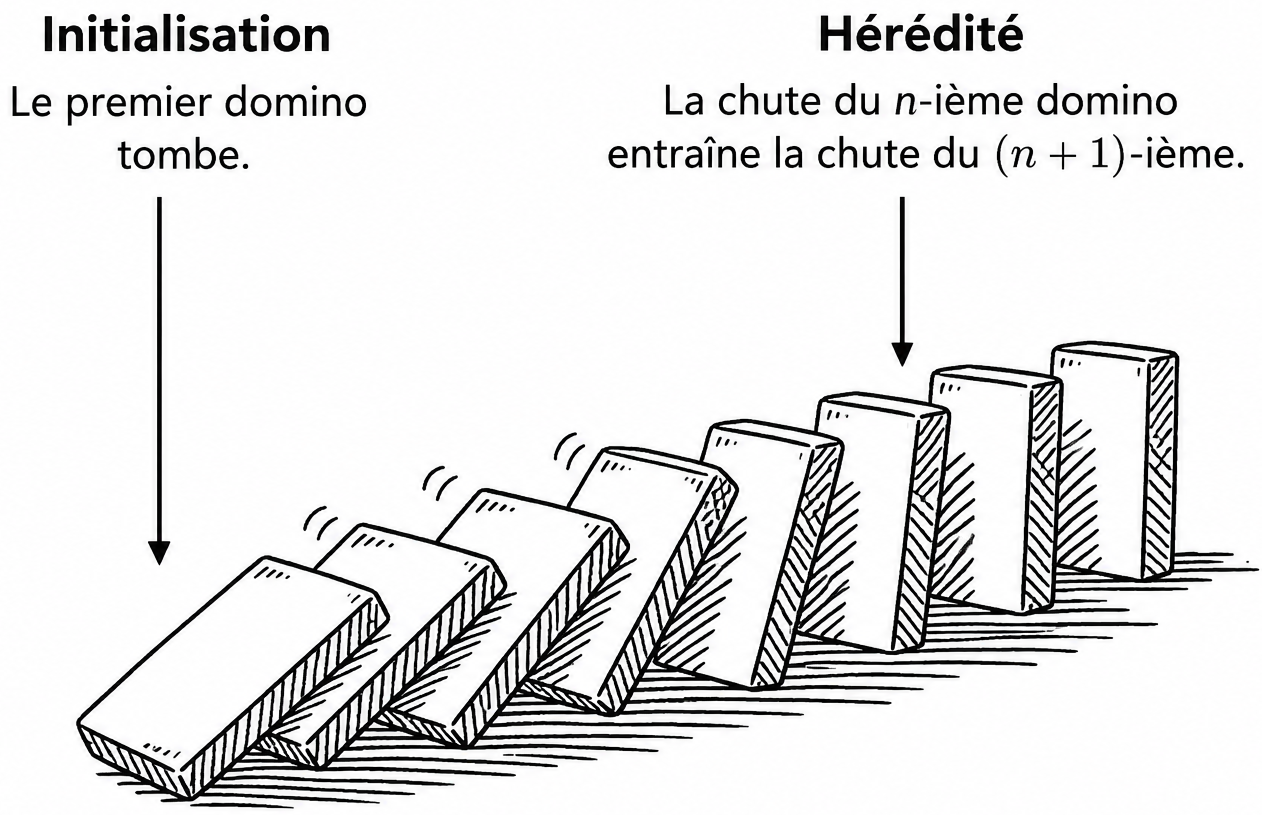
\includegraphics[width=\linewidth]{figures/analyse/domino}	
\end{minipage}
\subsection{Principe du raisonnement par récurrence}
\begin{theoreme}[Principe de récurrence]
	
Soit $P(n)$ une propriété qui dépend d'un nombre naturel $n$ et
$n_0$ un entier naturel fixé.

Si la propriété $P(n)$ vérifie les deux conditions suivantes :

\begin{enumerate}
	\item \textbf{Initialisation :} $P(n_0)$ est vraie ;
	
	\item \textbf{Hérédité :} si $P(k)$ est vraie pour un entier naturel
	$k \geq n_0$, alors $P(k+1)$ est vraie
\end{enumerate}

alors, \textbf{pour tout entier naturel $n \geq n_0$},
$P(n)$ est vraie.
\end{theoreme}

\remarque 
\begin{itemize}
	
	\item La propriété $P(n)$ peut être une égalité, une inégalité, une propriété exprimée par une phrase, \ldots
	
	\item La condition d'hérédité est une implication : on suppose que
	$P(k)$ est vraie pour un nombre entier naturel $k$ supérieur ou égal à
	$n_0$ (c'est \textbf{l'hypothèse de récurrence}) et on montre qu'alors
	$P(k+1)$ est vraie elle aussi.
	
	Une propriété $P(n)$ qui vérifie cette deuxième condition est dite
	héréditaire à partir du rang $n_0$ ; en effet, elle se transmet du nombre entier
	$k$ à son « successeur » $k+1$.
	
\end{itemize}

\begin{center}
	
\includegraphics[width=\textwidth]{analyse/resume_recurrence}
\end{center}

\exerciceresolu 
$(u_n)$ est la suite définie par $u_0=0$ et pour tout entier naturel $n, u_{n+1}=2u_n+1 $

Démontrer par récurrence que, pour tout entier naturel $u_n=2^n-1.$

\solution
\begin{itemize}[label=\textbullet]
	
	\item \textbf{Initialisation :} Pour $n=0$, $u_0=0$ et $2^0-1=0$. Ainsi $P(0)$ est vraie.
	
	\item \textbf{Hérédité :} Supposons $P(k)$ vraie, c'est-à-dire $u_k=2^k-1$ (hypothèse de récurrence).\\
	Démontrons qu'alors que $P(k+1)$ est vraie, c'est-à-dire que $u_{k+1}=2^{k+1}-1.$ \\
	Or, $u_{k+1}=2u_k+1$. Ainsi, d'après l'hypothèse de récurrence,
	$u_{k+1}=2(2^k-1)+1=2^{k+1}-1$.
	
	Alors
	$$
	u_{k+1}=2u_k+1
	=2(2^k-1)+1
	=2^{k+1}-1.
	$$
	
	Donc $P(k+1)$ est vraie.
	
	\item \textbf{Conclusion :} La propriété est vraie pour tout entier naturel $n$.
	
\end{itemize}


Sur le modèle de l'exercice résolu ci-dessus :
\exercice{\etoilepleine\etoilevide\etoilevide}
\begin{minipage}[t]{0.46\textwidth}
	
	\textbf{1)} $(v_n)$ est la suite définie par $v_0=0$ et
	$v_{n+1}=v_n+2n+2$.
	
	Démontrer par récurrence que, pour tout entier naturel $n$,
	$v_n=n(n+1)$.
	
\end{minipage}
\hfill
\vrule width 1pt
\hfill
\begin{minipage}[t]{0.46\textwidth}
	\textbf{2)} $(w_n)$ est la suite définie par $w_0=0$ et
	$w_{n+1}=2w_n-3$.
	
	Démontrer par récurrence que, pour tout entier naturel $n$,
	$w_n=3(1-2^n)$.
	
\end{minipage}





